\documentclass[UTF8,fontset=ubuntu]{ctexart}
\usepackage{tikz}
\usetikzlibrary{datavisualization.formats.functions}

% tikz作函数图的方式
%   1)\path plot
%   2)datavisualization
%   3)pgfplots package



% 1.plot
%   1)\path plot[<options>] coordinates {(<coordinate_1>) (coordinate_2) (coordinate_3)...}
%   根据坐标点作图
\begin{tikzpicture}
    \draw plot coordinates {(0,0) (1,0) (2,1) (3,0)};
\end{tikzpicture}

%   2)\path plot[<options>] file {<file_name>}

%   3)\path plot[<options>] <coordinate_expression>
%   根据坐标点表达式作图. 相关参数:
%     [1]variable=<macro>
%       使用的变量. 默认为\x
%     [2]samples=<number>
%       取样本数量
%     [3]domain=<start>:<end>
%       变量的取值范围
%     [4]samples at=<samples_list>
%       样本取值列表
%     [5]smooth
%       使用曲线连接
\begin{tikzpicture}[>=stealth]
    \draw[->] (-4,0) -- (4,0) node[below]{$x$};
    \draw[->] (0,-4) -- (0,4) node[left]{$y$};
    \draw[help lines] (-3,-3) grid (3,3);
    \draw plot[samples=100,domain=-3:3] (\x,\x);
\end{tikzpicture}

\begin{tikzpicture}[>=stealth]
    \draw[help lines] (-3,-3) grid (3,3);
    \draw[->] (-4,0) -- (4,0) node[below]{$x$};
    \draw[->] (0,-4) -- (0,4) node[left]{$y$};
    \draw plot[samples=200,domain=-pi:pi] (\x,{sin(\x r)});
\end{tikzpicture}

%   4)\path plot[options] function {<gnuplot_formula>}
    





% 1.datavisualization,参考section 82,第872页. 需要使用datavisualization库
\begin{document}
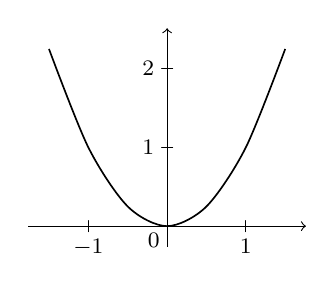
\begin{tikzpicture}
    % 使用坐标点作图
    \datavisualization [school book axes,visualize as smooth line]
    data {
      x,y
      -1.5,2.25
      -1,1
      -0.5,0.25
      0,0
      0.5,0.25
      1,1
      1.5,2.25
    };
\end{tikzpicture}\\\vspace{1cm}

\begin{tikzpicture}
  \datavisualization [
    % 使用函数方式作图,需要使用datavisualization.formats.functions库
    % 1.scientific axes
    % 科学坐标轴,值格式: {<key>=<value>}可指定以下值:
    %   1)outer ticks - 刻度放置在外部
    %   2)inner ticks - 刻度放置在内部
    %   3)clean - 不在原边框画刻度,分别在左侧和下侧建立坐标轴
    %   4)standard labels/upright labels/end labels - 坐标标签的放置方式. 放置方式如下:
    %     [1]standard labels - x轴标签在轴中间下方;y轴标签在轴中间左侧,文字从下到上
    %     [2]upright labels - x轴标签在轴中间在下方;y轴标签在周中间左侧,文字从左到右
    %     [3]end labels - x轴标签在轴末端右侧;y轴标签在轴末端上侧,文字从左到右
    scientific axes,
    % x axis代表x轴的相关参数. 可使用参数如下:
    %   1)attribute - 轴表示的含义, 如: 时间/速度等
    %   2)label - 轴标签. 值格式为: {[<options>]<text>}. 如: [below]$x$, 代表标签位于轴结束位置的下方
    %   3)include value - 坐标轴上必须包含的刻度. 还有类似指定最小刻度和最大刻度的关键字:
    %     [1]min value
    %     [2]max value
    %   4)logarithmic - 将数轴的刻度按指数进行递增
    %   5)length - 轴的实际长度
    %   6)unit length - 轴上步进num对应的长度, 值格式: <dimension> per <num> units
    %   7)power unit length - unit length的logarithmic版本
    %   8)ticks - 指定刻度相关. 值格式: {<key>=<value>}, key列表:
    %     [1]about - 大约指定tick个数
    %     [2]none/few/some/many - 分别代表无刻度、少量刻度(about=3)、适量刻度(about=5)、大量刻度(about=10)
    %     [3]step - 指定大刻度步进
    %     [4]minor steps between steps - 大刻度之间的小刻度数量
    %     [5]major at - 详细指定大刻度的所在值, 值格式: {<list>}
    %     [6]minor at - 详细指定小刻度的所在值, 值格式: {<list>}
    %     [7]subminor at - 详细指定更小刻度的所在值, 值格式: {<list>}
    %     [8]major/minor/subminor also at - 额外附加的刻度值
    %     [9]style - 对刻度线和刻度值进行配置
    %     [10]node style - 对刻度值进行配置,值格式: {<key>=<value>}. 如: 
    %         color=blue - 刻度值为蓝色
    %         yshift=2pt - 刻度值向上移动2pt
    %         rotate=90 - 刻度值旋转90度
    %         above/below/left/right - 刻度值相对于刻度的位置
    %     [11]tick prefix - 在刻度值前面添加的内容
    %     [12]tick suffix - 在刻度值后面添加的内容
    %     [13]tick unit - 刻度值的单位. 类似于tick suffix={$\,\rm<text>$}
    %     [14]stack - 刻度值进行错位显示(偶数项拉伸)
    %     [15]stack' - 刻度值进行错位显示(奇数项拉伸)
    x axis={label=$x$,ticks={major at={1,2,3},minor at={0.5,1.5,2.5},subminor at={0.25,0.75}}},
    y axis={label=$y$},

    % 线条类型:
    %   1)visualize as line - 直线
    %   2)visualize as smooth line - 曲线
    %   3)visualize as scatter - 描点
    % 可在线条类型中,指定使用该线条类型的线条,如果有多个线条,可以使用如下格式指定:
    %   visualize as line/.list={<line_name_01>,<line_name_02>,...}
    visualize as smooth line]

    % format - 提供坐标点的方式. 可选列表如下:
    %   1)table - 第一行为表头,后续行为内容;列之间的分隔符默认为','. 默认格式,使用如下参数修改子参数:
    %     [1]separator - 指定列之间的分隔符
    %     [2]headline - 指定表头名称,此时内容第一行为实际值
    %   2)named - 使用<var>=<val>的方式分别指定内容;列之间分隔符默认为','
    %   3)function - 使用函数表达内容,使用使用datavisualization.formats.functions库. 格式如下:
    %     [1]var <var> : interval[<low>:<high>] samples <num>
    %     samples为样本数,可省略,默认为25
    %     [2]var <var> : interval[<low>:<high>] step <step>
    %     [3]var <var> : {<values>}
    %     [4]func <var> = <expression>
    %     引用变量值: \value{<var>}
    data [format=function] {
      var x : interval [-3:3];
      func y = \value x*\value x*\value x;
    };
\end{tikzpicture}\\\vspace{1cm}

\begin{tikzpicture}
  % 2.school book axes,需要使用datavisualization
  \datavisualization [
    school book axes,
    visualize as smooth line,
    x axis={label=$x$},
    y axis={label=$f(x)$}]
    data [format=function] {
      var x : interval [-1.3:1.3];
      func y = \value x*\value x*\value x;
    };
\end{tikzpicture}\\\vspace{1cm}

\begin{tikzpicture}
  % 3.xy Cartesian,需要使用datavisualization
  \datavisualization [
    xy Cartesian,
    visualize as smooth line]
    data [format=function] {
      var x : interval [-1.3:1.3];
      func y = \value x*\value x*\value x;
    };
\end{tikzpicture}\\\vspace{1cm}

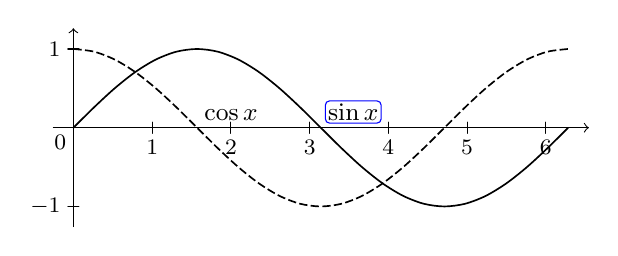
\begin{tikzpicture}
    % 在线条处插入标注
    \datavisualization [
    school book axes,
    visualize as smooth line/.list={sin,cos},
    % 对应线条的属性. 列表如下:
    %   1)label in data - 该线条注释文字的属性. 列表如下:
    %     [1]text - 注释文字内容, 位于线条右侧
    %     [2]text' - 注释文字内容, 位于线条左侧
    %     [3]when - 注释文字的放置点. 如: when=x is 2或when=y is 3
    %     [4]index - 注释文字位于数据集第num个点
    %     [5]pos - 注释文字在线条的百分比位置
    %     [6]node style - 配置标签属性. 如: node style={circle,draw=red}
    %     [7]text colored - 配置标签的颜色与线条一致
    sin={label in data={text=$\sin x$,node style={draw=blue},pos=0.5}},
    cos={label in data={text=$\cos x$,pos=0.25}},
    style sheet=vary dashing
    ]
    % set参数,指定该数据集用于指定线条
    data [set=sin,format=function]{
      var x : interval [0:2*pi];
      % r用于将弧度制x转化为角度制
      func y = sin(\value x r);
    }
    data [set=cos,format=function]{
      var x : interval [0:2*pi];
      % r用于将弧度制x转化为角度制
      func y = cos(\value x r);
    };
\end{tikzpicture}\\\vspace{1cm}

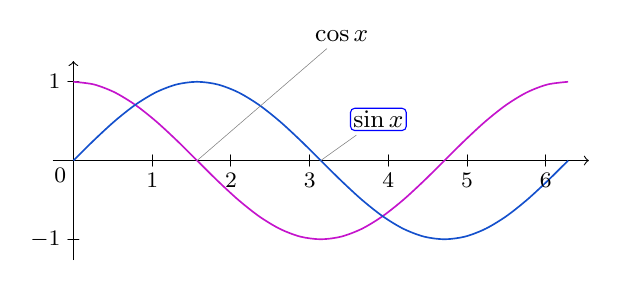
\begin{tikzpicture}
    % 在线条处插入标注,并连接
    \datavisualization [
    school book axes,
    visualize as smooth line/.list={sin,cos},
    % 对应线条的属性. 列表如下:
    %   1)pin in data - 该线条注释文字的属性. 列表如下:
    %     [1]text - 注释文字内容, 位于线条右侧
    %     [2]text' - 注释文字内容, 位于线条左侧
    %     [3]when - 注释文字的放置点. 如: when=x is 2或when=y is 3
    %     [4]index - 注释文字位于数据集第num个点
    %     [5]pos - 注释文字在线条的百分比位置
    %     [6]node style - 配置标签属性. 如: node style={circle,draw=red}
    %     [7]text colored - 配置标签的颜色与线条一致
    %     [8]pin angle - pin的角度
    %     [9]pin length - pin的长度
    sin={pin in data={text=$\sin x$,node style={draw=blue},pos=0.5}},
    cos={pin in data={text=$\cos x$,pos=0.25,pin length=2cm}},
    style sheet=vary hue
    ]
    % set参数,指定该数据集用于指定线条
    data [set=sin,format=function]{
      var x : interval [0:2*pi];
      % r用于将弧度制x转化为角度制
      func y = sin(\value x r);
    }
    data [set=cos,format=function]{
      var x : interval [0:2*pi];
      % r用于将弧度制x转化为角度制
      func y = cos(\value x r);
    };
\end{tikzpicture}\\\vspace{1cm}

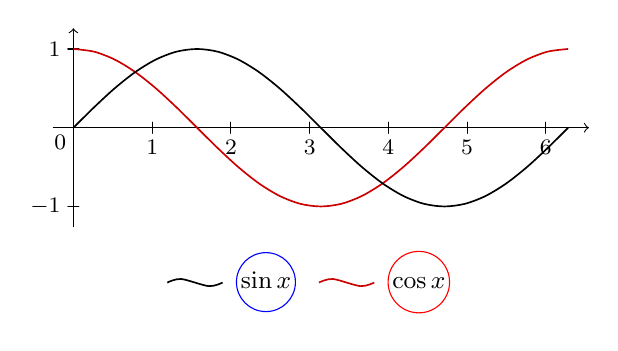
\begin{tikzpicture}
    % legend应用
    \datavisualization [
    school book axes,
    % legend - 配置legend相关属性. 列表如下:
    %   1)above - legend在坐标轴外部的位置. 可选列表如下:
    %     [1]east outside/right - 在右侧
    %     [2]north east outside - 在右上侧,并且顶端与可视表的顶端对齐
    %     [3]south east outside - 在右下侧,并且底端与可视表的底端对齐
    %     [4]west outside/left - 在左侧
    %     [5]north west outside - 在左上侧,并且顶端与可视表的顶端对齐
    %     [6]south west outside - 在左下侧,并且底端与可视表的底端对齐
    %     [7]north outside/above - 在顶侧
    %     [8]south outside/below - 在底侧
    %   2)east inside - legend在坐标轴内部的相对位置. 可选列表如下:
    %     [1]east inside - 内部右侧
    %     [2]north east inside - 内部右上侧
    %     [3]south east inside - 内部右下侧
    %     [4]west inside - 内部左侧
    %     [5]north west inside - 内部左上侧
    %     [6]south west inside - 内部左下侧
    %     [7]north inside - 内部上侧
    %     [8]south inside - 内部下侧
    %   3)at values - legend在坐标轴内部的坐标点位置. 可选列表如下:
    %     [1]at values - legend的中心的坐标点. 格式: at values={x=<val>,y=<val>}
    %     [2]right of - legend的中心在坐标点的右侧
    %     [3]above right of - legend的中心在坐标点的右上侧
    %     [4]above of - legend的中心在坐标点的上侧
    %     [5]above left of - legend的中心在坐标点的左上侧
    %     [6]left of - legend的中心在坐标点的左侧
    %     [7]below left of - legend的中心在坐标点的左下侧
    %     [8]below of - legend的中心在坐标点的下侧
    %     [9]below right of - legend的中心在坐标点的右下侧
    %   4)matrix node style - legend矩阵的属性. 如: fill=black!50
    %   5)down then right - legend的内容,排序方式. 列表如下:
    %     [1]down then right - 先从上到下,再从左到右. 默认选项
    %     [2]down then left - legend的内容,先从上到下,再从右到左
    %     [3]up then right - legend的内容,先从下到上,再从左到右
    %     [4]up then left - legend的内容,先从下到上,再从右到左
    %     [5]left then up - legend的内容,先从右到左,再从下到上
    %     [6]left then down - legend的内容,先从右到左,再从上到下
    %     [7]right then up - legend的内容,先从左到右,再从下到上
    %     [8]right then down - legend的内容,先从左到右,再从上到下
    %   6)rows - legend的行数
    %   7)columns - legend的列数
    %   8)label style - 配置legend标签的属性. 列表如下:
    %     [1]node style - 配置标签属性. 如: node style={circle,draw=red}
    %     [2]text colored - 配置标签的颜色与线条一致
    %     [3]text right - 标签放置在线条的相对位置. 列表如下:
    %       1]text right - 标签放在线条右侧. 默认配置
    %       2]text left - 标签放在线条左侧
    %       3]text only - 只有标签, 没有线条
    legend={below,label style={node style={draw=red,circle}}},
    visualize as smooth line/.list={sin,cos},
    % 对应线条的属性. 列表如下:
    %   1)label in legend - legend中该线条注释文字的属性. 列表如下:
    %     [1]text - 注释文字内容
    %     [2]node style - 线条在legend的标签属性. 如: node style={circle,draw=blue}
    %   2)style - 线条在坐标轴中的属性. 列表如下:
    %     [1]<color> - 指定线条颜色
    %     [2]mark - 指定标记点的形状
    sin={label in legend={text=$\sin x$,node style={draw=blue}}},
    cos={label in legend={text=$\cos x$}},
    % style sheet指定不同线条的区分方式. 列表如下:
    %   1)vary dashing - 通过线条dash模式来区别线条
    %   2)vary thickness - 通过线条粗细来区别线条
    %   3)vary thickness and dashing - 通过线条粗细和dash模式来区别线条
    %   4)cross marks - 使用不同的标记来区别线条或scatter
    %   5)strong colors - 使用不同主色来区别线条
    %   6)vary hue - 使用不同颜色来区别线条
    %   7)shades of blue - 使用不同深浅的蓝色来区别线条
    %   8)shades of red - 使用不同深浅的红色来区别线条
    %   9)gray scale - 使用不同灰度来区别线条
    style sheet=strong colors
    ]
    % set参数,指定该数据集用于指定线条
    data [set=sin,format=function]{
      var x : interval [0:2*pi];
      % r用于将弧度制x转化为角度制
      func y = sin(\value x r);
    }
    data [set=cos,format=function]{
      var x : interval [0:2*pi];
      % r用于将弧度制x转化为角度制
      func y = cos(\value x r);
    };
\end{tikzpicture}\\\vspace{2cm}

% 修改默认箭头>为latex模式
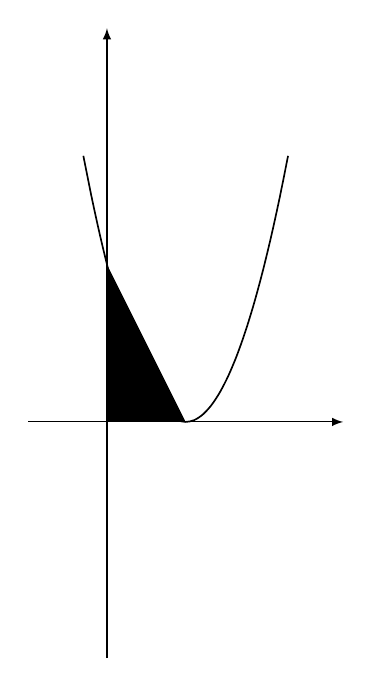
\begin{tikzpicture}[>=latex]
    \datavisualization[
        xy Cartesian,
        visualize as smooth line
    ]
    data [format=function]{
        var x : interval[-0.3:2.3];
        func y = 2*(\value x-1)*(\value x-1);
    };
    \draw[->] (-1,0) -- (3,0);
    \draw[->] (0,-3) -- (0,5);
    \fill (1,0) -- (0,0) -- (0,2);
\end{tikzpicture}\\\vspace{4mm}



\end{document}
